\chapter{提案手法}
\label{proposed}

本章では提案手法について述べる.

\section{概要}
~\ref{issue}章で述べた仮説を検証するために,本研究の手法について解説する.

\subsection{問題解決の為のアプローチ}
本手法ではQRコードの中心を原点とした座標系でドローンは自己位置推定を行う.
この時,QRコードのデータ部をデコードし,同時に経路情報を取得する.\ref{flow_sample}

データ部には以下のフォーマットでデータが格納されており,
観測しているQRコード座標系での次に向かうべきQRコードの座標データが記載されている.
また,本システムで扱う距離単位は全てcm(センチメートル)である.
\begin{lstlisting}[caption=data format,label=data_format]
{
  "x"?: number;
  "y"?: number;
  "z"?: number;
  "rotate"?: number;
  "command"?: string;
}
\end{lstlisting}
\begin{figure}[htbp]
  \begin{center}
    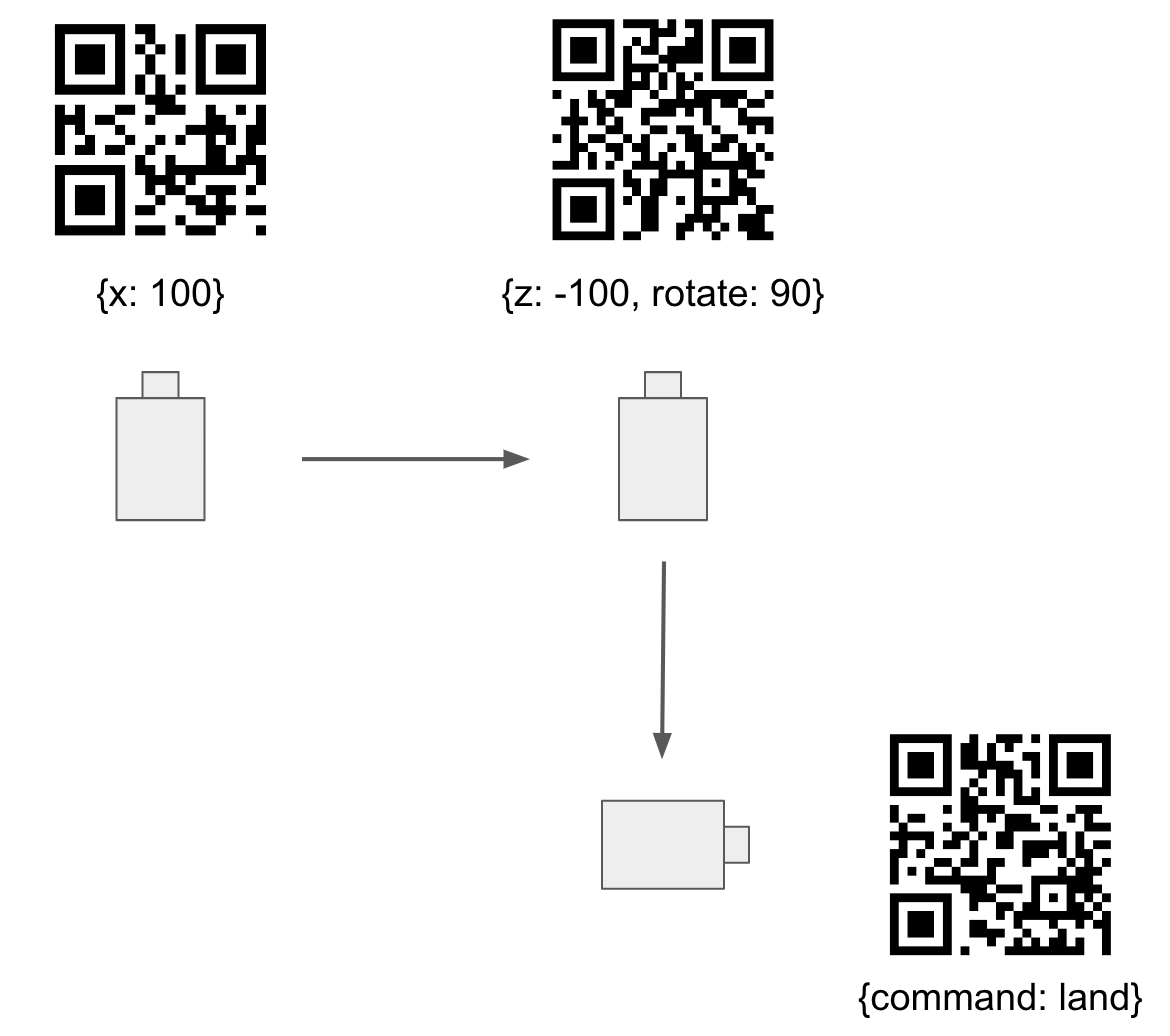
\includegraphics[clip,width=15.0cm]{img/flow.png}
    \caption{ナビゲーション時の簡略図}
    \label{flow_sample}
  \end{center}
\end{figure}


%%% Local Variables:
%%% mode: japanese-latex
%%% TeX-master: "../bthesis"
%%% End:
